\documentclass[tikz,border=5pt]{standalone}
\usepackage{fontspec}
\setmainfont{Times New Roman}
\usepackage{unicode-math}
\setmathfont{Cambria Math}
\usetikzlibrary{shapes.geometric,positioning,fit,backgrounds,arrows.meta,calc}

\begin{document}
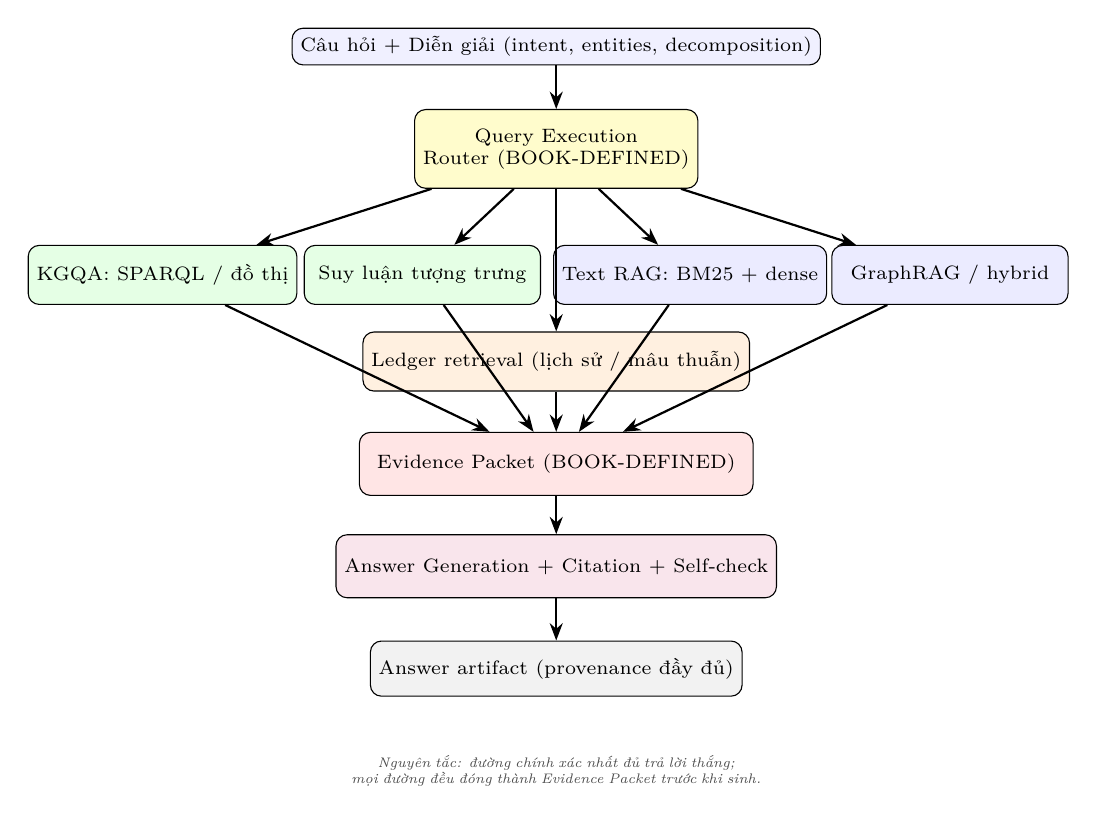
\begin{tikzpicture}[
  box/.style={rectangle, draw, rounded corners, align=center, font=\scriptsize, inner sep=3pt},
  pathbox/.style={box, minimum width=3.0cm, minimum height=0.75cm},
  arrow/.style={-{Stealth[length=2.2mm]}, thick},
  label/.style={font=\tiny\itshape, text=gray!60!black},
]

% === Input ===
\node[box, fill=blue!6, minimum width=5cm] (in) at (0, 5.2) {Câu hỏi + Diễn giải (intent, entities, decomposition)};

% === Router ===
\node[box, fill=yellow!20, minimum width=3.0cm, minimum height=1.0cm] (router) at (0, 3.9) {Query Execution\\Router (BOOK-DEFINED)};

\draw[arrow] (in) -- (router);

% === Paths (y = 2.3) ===
\node[pathbox, fill=green!10] (p1) at (-5.0, 2.3) {KGQA: SPARQL / đồ thị};
\node[pathbox, fill=green!10] (p2) at (-1.7, 2.3) {Suy luận tượng trưng};
\node[pathbox, fill=blue!8] (p3) at (1.7, 2.3) {Text RAG: BM25 + dense};
\node[pathbox, fill=blue!8] (p4) at (5.0, 2.3) {GraphRAG / hybrid};

\draw[arrow] (router) -- (p1);
\draw[arrow] (router) -- (p2);
\draw[arrow] (router) -- (p3);
\draw[arrow] (router) -- (p4);

% === Ledger retrieval (below center) ===
\node[pathbox, fill=orange!12] (p5) at (0, 1.2) {Ledger retrieval (lịch sử / mâu thuẫn)};
\draw[arrow] (router) -- (p5);

% === Evidence Packet ===
\node[box, fill=red!10, minimum width=5cm, minimum height=0.8cm] (ep) at (0, -0.1) {Evidence Packet (BOOK-DEFINED)};

\draw[arrow] (p1) -- (ep);
\draw[arrow] (p2) -- (ep);
\draw[arrow] (p3) -- (ep);
\draw[arrow] (p4) -- (ep);
\draw[arrow] (p5) -- (ep);

% === Answer Synthesis ===
\node[box, fill=purple!10, minimum width=4.4cm, minimum height=0.8cm] (syn) at (0, -1.4) {Answer Generation + Citation + Self-check};

\draw[arrow] (ep) -- (syn);

% === Answer artifact ===
\node[box, fill=gray!10, minimum width=3.8cm, minimum height=0.7cm] (aa) at (0, -2.7) {Answer artifact (provenance đầy đủ)};

\draw[arrow] (syn) -- (aa);

% === Principle ===
\node[label, align=center, text width=11cm] at (0, -4.0)
  {Nguyên tắc: đường chính xác nhất đủ trả lời thắng;\\mọi đường đều đóng thành Evidence Packet trước khi sinh.};

\end{tikzpicture}
\end{document}